\section*{Problem 2}

Consider the network fragment shown in Figure 1.
$x$ has two attached neighbours, $w$ and $y$
$w$ has a minimum-cost path to destination $u$ (not shown) of 5 and $y$ has a minimum-cost path to $u$ of 6.
The complete path from $w$ and $y$ to $u$ (and between $w$ and $y$) are not shown.
All link costs in the network have strictly positive integer values.

\begin{enumerate}
    \item Give $x$ distance vector for destination $w$, $y$, and $u$.
    \item Give a link cost change for either $c(x, w)$ or $c(x, y)$ such that $x$ will inform its neighbor of a new minimum cost path to $u$ as a result of executing the distance-vector algorithm.
    \item Give a link-cost change for either $c(x, w)$ or $c(x, y)$ such that $x$ will not inform its neighbors of a new minimum cost path to $u$ as a result of executing the distance-vector algorithm.
\end{enumerate}

\begin{figure}[H]
    \centering
    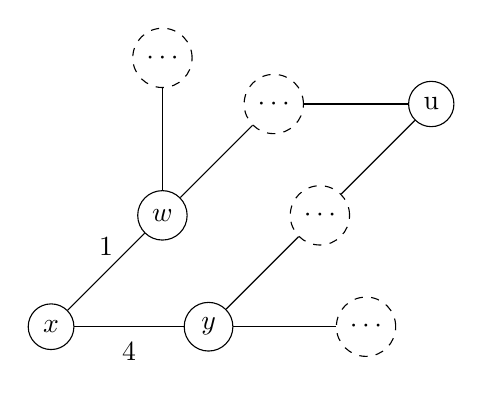
\begin{tikzpicture}
        \tikzstyle{every node} = [align=center, draw, circle, node distance = 2cm]
        \node(x){$x$};
        \node[above right of=x](w){$w$};
        \node[above right of=w, dashed](w1){$\cdots$};
        \node[above of=w, dashed](w2){$\cdots$};
        \node[right of=x](y){$y$};
        \node[above right of=y, dashed](y1){$\cdots$};
        \node[right of=y, dashed](y2){$\cdots$};
        \node[above right of=y1](u){u};

        \path (x) edge node[draw=none, above](){1} (w);
        \path (x) edge node[draw=none, below](){4} (y);
        \path (w) edge (w1);
        \path (w) edge (w2);
        \path (y) edge (y1);
        \path (y) edge (y2);
        \path (y1) edge (u);
        \path (w1) edge (u);
    \end{tikzpicture}
    \caption{Fragment of a network}
\end{figure}

\subsection*{Solution}

\begin{enumerate}
    \item The vector is shown below:
          \begin{table}[H]
              \centering
              \begin{tabular}{lllll}
                  From $x$ & Via $x$ & Via $y$ & Via $w$ & Via $u$ \\
                  To $x$   & -       & -       & -       & -       \\
                  To $y$   & -       & 4       & 12      & NA      \\
                  To $w$   & -       & 15      & 1       & NA      \\
                  To $u$   & -       & 10      & 6       & NA
              \end{tabular}
          \end{table}
    \item If we change $c(x, y)$ to $0$, then $x$ has to inform $y$ that the new shortest from $y$ to $u$ is via $x$.
    \item If we change $c(x, w)$ to $2$, nothing needs to be changed.   
\end{enumerate}